\section{Sch\"{a}r mountain waves}
\TODO{
\begin{itemize}
	\item Meshes: BTF, cut cell, slanted cell
	\item Schemes: linearUpwind, cubicFit
	\item Plot: incorrect w contours using linearUpwind, compare with Melvin et al. 2010
	\item Plot: theta diff heatmap
	\item Plot: schaerWaves and thermalAdvect vertical cross-sections of theta diff
	\item Conclusion: unlike linearUpwind, cubicFit gives the correct solution (at least on BTF? is linearUpwind better on cut/slanted cells?)
	\item Conclusion: should we test max(dt) again? we've not yet done so for a dynamical test.  I'd hope that slanted cells are much better than cut cells.
\end{itemize}
}

\begin{figure}
	\centering
	\begin{subfigure}{0.48\textwidth}
		% TODO: move this subfigure into its own pdf and annotate GmtPlot axes
		\centering
		\includegraphics{schaerWaves-btf-300dz-linearUpwind/18000/w.pdf}
		\TODO{linearUpwind}
	\end{subfigure}
	\begin{subfigure}{0.48\textwidth}
		\centering
		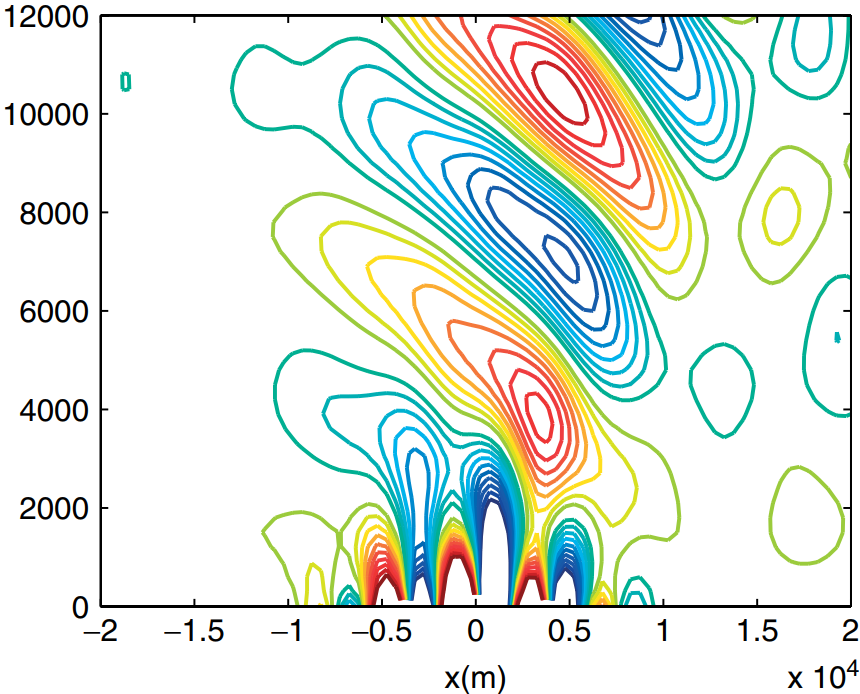
\includegraphics[height=2in]{slanted/schaerWaves/melvin2010-w-mass-conserving-sisl.png}
		\caption{\citep{melvin2010}}
		\label{fig:slanted:schaerWaves:w:melvin}
	\end{subfigure}
	\caption{\TODO{$w$ contours}}
	\label{fig:slanted:schaerWaves:w}
\end{figure}

